\subsection{Elektronen in Festkörpern: Bänder, Metalle und Halbleiter}
\label{subsec:elektronen-festkoerper-baender-metalle-halbleiter}

In einzelnen Atomen besitzen Elektronen diskrete Energieniveaus. Auch in
Molekülen entstehen durch die Überlagerung von Atomorbitalen neue
Molekülorbitale. In einem Festkörper\index{Festkörper} wird diese Idee noch
weitergeführt: Sehr viele Atome liegen regelmäßig oder nahezu regelmäßig
nebeneinander. Ihre Elektronenzustände beeinflussen sich gegenseitig.

Wenn viele Atome zu einem Kristall\index{Kristall} oder Festkörper
zusammenkommen, spalten sich die ursprünglich diskreten atomaren Energieniveaus
in sehr viele dicht beieinanderliegende Zustände auf. Bei einer großen Zahl von
Atomen erscheinen diese Zustände nicht mehr als einzelne Linien, sondern als
Energiebänder\index{Energieband}.

Damit entsteht ein neues Bild: Elektronen in Festkörpern werden nicht mehr nur
einzelnen Atomen zugeordnet. Sie können Zustände einnehmen, die sich über viele
Atome hinweg erstrecken. Genau diese Bandstruktur bestimmt, ob ein Stoff ein
Metall\index{Metall}, ein Halbleiter\index{Halbleiter} oder ein Isolator
\index{Isolator} ist.

\begin{PhysicsBox}[Energiebänder im Festkörper]
	\label{box:energiebaender-im-festkoerper}
	In einem einzelnen Atom besitzen Elektronen diskrete Energieniveaus. In einem
	Festkörper wechselwirken sehr viele Atome miteinander. Dadurch spalten sich
	die atomaren Energieniveaus in viele eng benachbarte Zustände auf.
	
	Diese dicht liegenden Zustände bilden Energiebänder. Die Anordnung und
	Besetzung dieser Bänder bestimmt die elektrischen Eigenschaften eines
	Festkörpers.
\end{PhysicsBox}

Besonders wichtig sind zwei Begriffe: das Valenzband\index{Valenzband} und
das Leitungsband\index{Leitungsband}. Das Valenzband enthält Elektronen, die
noch stark zur Bindung im Festkörper beitragen. Das Leitungsband enthält
Zustände, in denen Elektronen sich leichter durch den Festkörper bewegen
können. Zwischen beiden kann eine Energielücke liegen, die man Bandlücke
\index{Bandlücke} nennt.
\FloatBarrier
\begin{figure}[H]
	\centering
	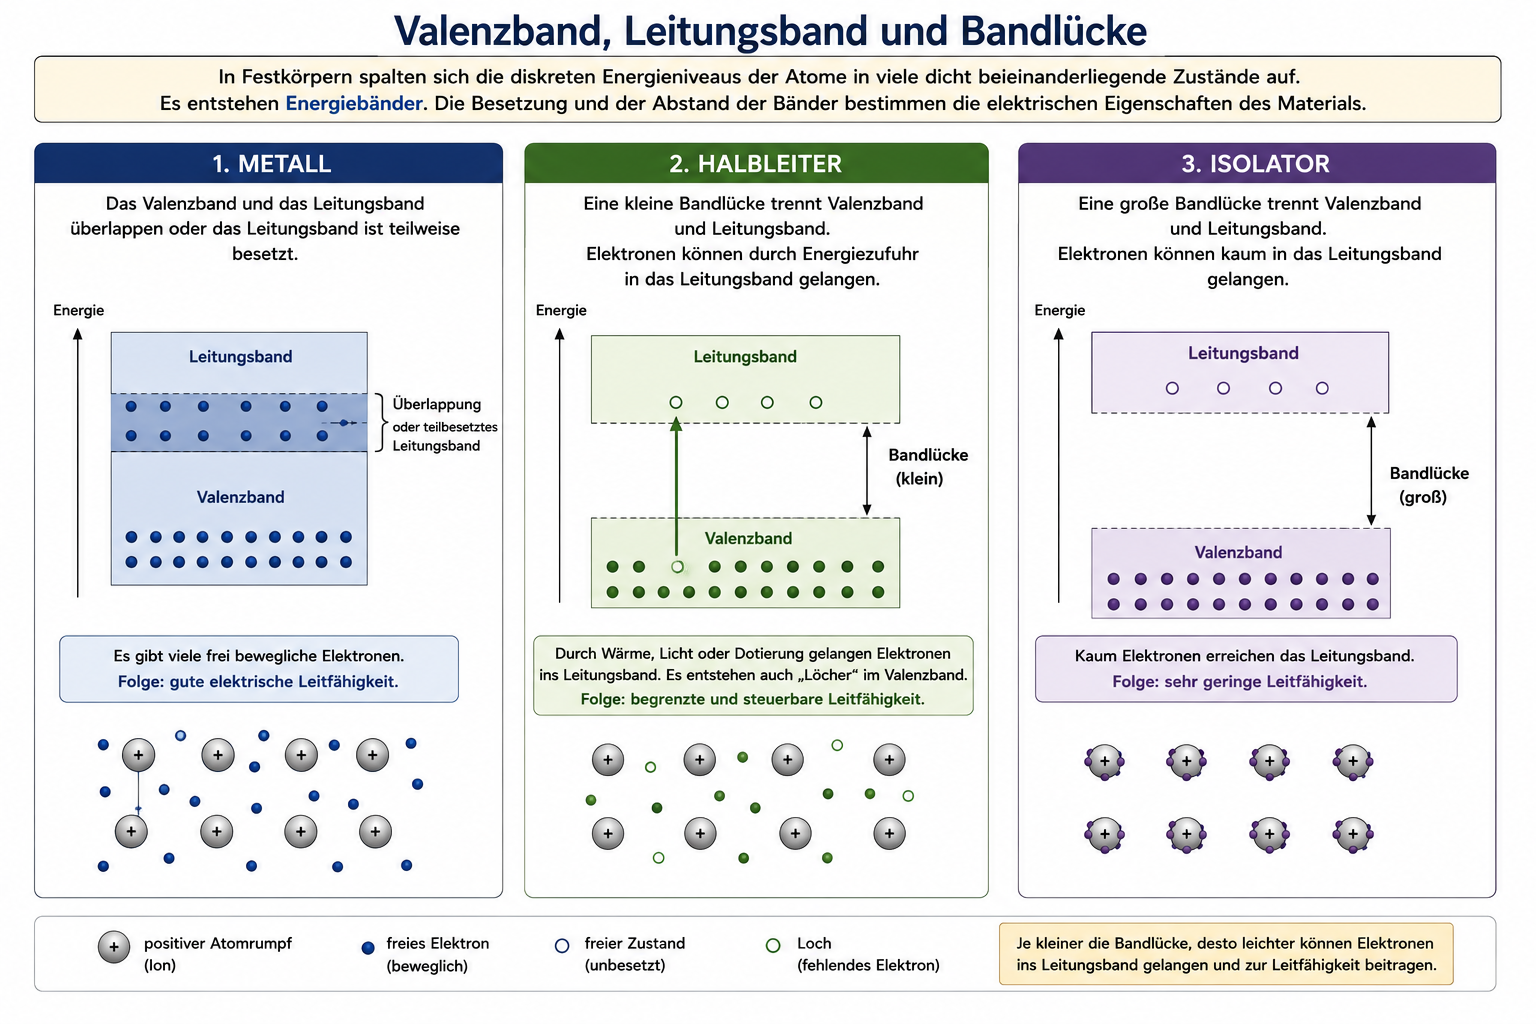
\includegraphics[width=0.85\textwidth]{bilder/Valenzband.png}
	\caption{Schematische Darstellung von Valenzband, Leitungsband und Bandlücke.
		Das Valenzband enthält die besetzten Elektronenzustände niedrigerer Energie.
		Das Leitungsband enthält Zustände, in denen Elektronen zur elektrischen
		Leitfähigkeit beitragen können. Die Bandlücke gibt die Energie an, die ein
		Elektron überwinden muss, um vom Valenzband in das Leitungsband zu gelangen.}
	\label{fig:valenzband-leitungsband-bandluecke}
\end{figure}
Bei Metallen ist das Leitungsband teilweise besetzt oder überlappt mit dem
Valenzband. Dadurch stehen bewegliche Elektronen zur Verfügung. Schon bei
kleinen elektrischen Feldern können sie eine gerichtete Bewegung überlagern.
Das erklärt die gute elektrische Leitfähigkeit von Metallen.

Bei Isolatoren ist die Bandlücke sehr groß. Die Elektronen im Valenzband können
nicht ohne Weiteres in das Leitungsband gelangen. Deshalb stehen kaum freie
bewegliche Ladungsträger zur Verfügung. Der Stoff leitet elektrischen Strom
nur sehr schlecht.

Halbleiter liegen zwischen diesen beiden Fällen. Ihre Bandlücke ist kleiner
als bei Isolatoren. Durch Wärme, Licht oder gezielte Verunreinigungen können
Elektronen in das Leitungsband gelangen. Dann entstehen bewegliche
Ladungsträger. Genau diese Steuerbarkeit macht Halbleiter zur Grundlage der
modernen Elektronik.

\begin{DidacticBox}[Metall, Isolator und Halbleiter]
	\label{box:metall-isolator-halbleiter}
	Der Unterschied zwischen Metall, Isolator und Halbleiter liegt nicht einfach
	darin, ob Elektronen vorhanden sind. Elektronen gibt es in allen Stoffen.
	
	Entscheidend ist, ob Elektronen leicht bewegliche Zustände erreichen können:
	\begin{itemize}
		\item In Metallen stehen bewegliche Elektronen leicht zur Verfügung.
		\item In Isolatoren verhindert eine große Bandlücke den Ladungstransport.
		\item In Halbleitern kann die Leitfähigkeit gezielt beeinflusst werden.
	\end{itemize}
\end{DidacticBox}

Die klassische Vorstellung frei beweglicher Elektronen in einem Metall liefert
bereits eine erste Erklärung für elektrische Leitfähigkeit. Das Drude-Modell
\index{Drude-Modell} beschreibt Metalle anschaulich als ein Gitter positiver
Atomrümpfe, in dem sich Elektronen bewegen. Wird ein elektrisches Feld
angelegt, erhalten die Elektronen zusätzlich zu ihrer ungeordneten Bewegung
eine kleine gerichtete Driftbewegung. Diese Driftbewegung erzeugt den
elektrischen Strom.

Dieses Modell ist technisch nützlich, aber nicht vollständig. Es erklärt
anschaulich, warum Metalle leiten, verfehlt aber viele feinere Eigenschaften
von Festkörpern. Erst die Bandstruktur liefert eine tiefere Erklärung dafür,
warum manche Stoffe gute Leiter, andere Isolatoren und wieder andere
Halbleiter sind.

Für Halbleiter ist besonders wichtig, dass ihre Leitfähigkeit veränderbar ist.
Durch Dotierung\index{Dotierung} können gezielt Fremdatome eingebracht werden,
die zusätzliche Elektronen bereitstellen oder Elektronenlücken erzeugen. Diese
Elektronenlücken werden Löcher\index{Loch} genannt und verhalten sich im
elektrischen Feld wie positive Ladungsträger. Damit wird es möglich,
elektrischen Strom in Halbleitern gezielt zu steuern.

Genau diese Steuerbarkeit ist die Grundlage von Dioden, Transistoren und
integrierten Schaltungen. Ohne das Verhalten der Elektronen in Festkörpern
gäbe es keine moderne Elektronik, keine Computerchips und keine heutige
Informationstechnologie.

\begin{PhysicsBox}[Warum Halbleiter so wichtig sind]
	\label{box:warum-halbleiter-wichtig-sind}
	Halbleiter sind deshalb so bedeutend, weil ihre elektrische Leitfähigkeit
	gezielt verändert werden kann. Durch Dotierung, elektrische Felder oder Licht
	lassen sich bewegliche Ladungsträger erzeugen und steuern.
	
	Damit wird das Elektron im Festkörper zum aktiven Träger moderner
	Informationstechnik.
\end{PhysicsBox}

Der Blick auf Elektronen in Festkörpern zeigt, wie weit die Bedeutung des
Elektrons reicht. Es bestimmt nicht nur die Struktur einzelner Atome und
Moleküle, sondern auch die elektrischen Eigenschaften ganzer Materialien. Von
der chemischen Bindung bis zur Halbleitertechnik bleibt das Elektron der
entscheidende Akteur.

Damit ist der Übergang von der Elektronenhülle zur Materie vollzogen. Im
nächsten Kapitel wird der Blick wieder stärker historisch und atomphysikalisch:
Dort geht es um die Atommodelle und die Frage, wie das Elektron im Atom
verstanden wurde.